\documentclass[a4paper,12pt]{report}
\usepackage{graphicx}
\usepackage[backend=bibtex]{biblatex}
\usepackage[strings]{underscore}
\usepackage[T1]{fontenc}
\usepackage{amsmath}
\bibliography{dissertation}
\begin{document}
\title{Writing a Program to Evaluate Lambda Expressions}
\author{Yola Jones}
\date{\today}
\maketitle

\chapter{Design and Implementation}
\section{Design}

The overall program is split into a number of distinct elements. A grammar is used to define the syntax of a lambda term. Antlr is used to turn this grammar into an abstract syntax tree, which is used by an expression evaluator to traverse the tree and determine the result of the input lambda term.

A web interface is used to house this program, providing the user with a convenient and simple way to interact with the program.

Since Antlr is used to turn the grammar into an abstract syntax tree, this will not be documented in the design section, as this process has already been well-defined and will not be deviated from \cite{Parr2012}. However, the grammar, expression evaluator and the web interface are key blocks which need to be implemented with key factors in mind, and so have been discussed below. 

\subsection{Grammar}

The key aim in creating this grammar is creating a syntax which sticks as closely as possible to the rules of lambda calculus. Lambda Calculus grammar is already clearly defined, with a lambda term being either a variable, an abstraction or an application \cite{Hankin2004}. Applied lambda calculus adds functions and constants to this definition \cite{Slonneger1995}. Therefore the grammar of a lambda calculus term becomes:

\begin{itemize}
\item[|] Application (of form \texttt{[term] [term]}
\item[|] Abstraction (of form \texttt{[abstraction_term].[term]} where \texttt{[abstraction_term]} is of the form \texttt{$\lambda$[variable]})
\item[|] Function (of form \texttt{[term] [operation] [term]})
\item[|] Value (of form \texttt{[variable]} (the letters a-z) or \texttt{[number]} (constant))
\end{itemize}

With the addition of types, the grammar adds the option of a \texttt{:[type]} term to each variable, with each type being either a ground type (bool, int or none), or in the form \texttt{[type]->[type]}. This follows the standard syntax for typing used in the lecture material \cite{Hankin2004} \cite{Gay2019}, and will allow each student to input a lambda term directly from the lecture slides with minimal adjustment.

\subsection{Expression Evaluator}

The fundamental idea behind this evaluator is tree traversal, which navigates through the token nodes and performs different operations depending on the type of token encountered. For example, application tokens in the form MN will pass the right-hand term N to the left-hand term M. Abstractions will take the incoming value and substitute it into its own function. This will allow an evaluated expression to be built up, and a result evaluated.

Antlr provides two mechanisms for traversing an abstract syntax tree: listeners and visitors.

A listener is a passive way of evaluating a syntax tree, an antlr Walker object is declared alongside the desired listener class, the walker traverses the tree using a depth-first approach, triggering methods from the listener as it enters and exits each token \cite{Parr2012}. These listener methods can’t return values, so expressions and evaluations are to be handled using separate objects within the listener class. As the walker traverses the tree, the listener builds up a running evaluation of the term, returning the result when it exits the topmost node \cite{Srivastav2017}.

The key difference between a listener and a visitor is that a visitor controls its own traversal of the tree. By visiting the children of the current node explicitly, the path they take around the tree can be controlled \cite{Parr2012}, for example some children not being visited until their parents are evaluated, or a right-hand child being visited and evaluated before the left.

Visitors also allow custom return types, meaning rather than having to rely on separate objects for expression value return, nodes can return their resultant expressions directly to their parent node \cite{Srivastav2017}.

With beta reduction, different methods evaluate terms in different ways. In an application MN using a call-by-value approach, N is evaluated before M. In a call-by-need approach, N is passed into M before being evaluated.

This means that depending on the type of reduction selected, the evaluator will have to traverse the tree in a different order, suggesting visitor being more appropriate for this task than a listener. This is supported by the fact that when evaluating expressions, the evaluation will be happening as the tree is visited, and therefore there will be a great deal of return values needed. Having a separate object for storing these values could get complex, and so the visitor methods being able to return values directly to their parents will be more convenient for this task.

The visitor therefore will be the main code written in this project. A parser will be passed to a custom visitor interface, with different visitors being defined for each of the beta-reduction methods being implemented, since these methods will each traverse the tree in a different way.

The visitor should return tree things upon returning to the topmost node: the value of the expression, whether or not the term is typable, and what type the expression will be. It will also return details of any errors, for example syntax or “normal form does not exist” errors where applicable.

\subsection{Web Interface}

The web interface will allow the user to input a lambda term, along with the types of any terms. It will also allow the user to select which reduction strategy they would like to have the term evaluated by, with call-by-need (or normal order reduction) being selected as the default.

After the user has entered the data, a HTTP POST request will be used to send the data through the back-end code, which will process the term and return the result, type validity and the type of the final term from the visitor. This will then get displayed back to the user.

The layout should be simple and uncluttered, and should be suitable for those with a visual impairment.

\section{Implementation}

\subsection{Grammar}

The lambda grammar is contained in a .g4 file which defines the parser and lexer rules for lambda calculus, as required by Antlr. A section of the grammar is shown in \ref{parser_rules}, and indicates the parser rules for the term, application and abstraction token nodes, alongside the lexer rules in \ref{lexer_rules}.

\begin{figure}[p]
\centering
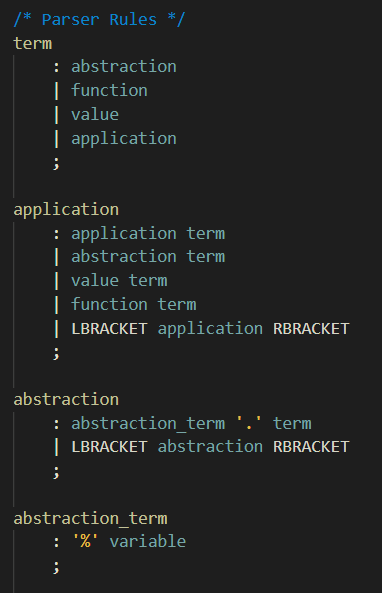
\includegraphics{images/parser_rules}
\caption{Parser Rules}
\label{parser_rules}
\end{figure}

\begin{figure}[p]
\centering
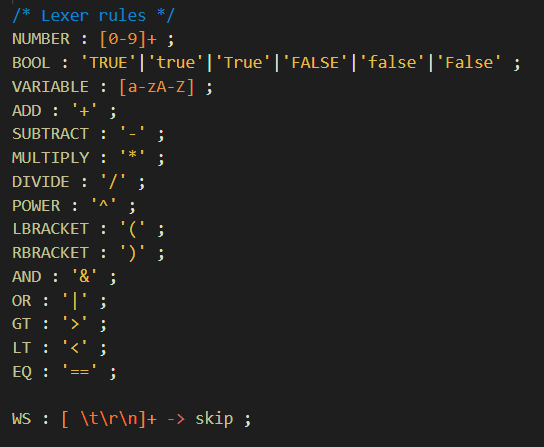
\includegraphics{images/lexer_rules}
\caption{Lexer Rules}
\label{lexer_rules}
\end{figure}

\subsection{Abstract Syntax Tree}

Having defined a grammar, antlr can then be used to create an abstract syntax tree. This is very simple to do, and involves passing the input term through an Input Stream class which converts this to a string of characters, then feeding this into a lexer (which outputs a set of tokens), a class which converts the tokens into an indexable list, and finally passing this through a parser which turns the tokens into an abstract syntax tree which can be explored \cite{Tomassetti2007}. This process is well documented and therefore will not be deviated from.
%screenshots needed here

\subsection{Expression Evaluator}
This is the largest block of code in the program, and defines how the incoming lambda term should be evaluated depending on the input given by the user. This code can be split into three distinct sections as discussed in the Background chapter of this report: alpha conversion, beta reduction and typing rules.

\subsubsection{Alpha Conversion}
The alpha conversion is based on the rules for explicit alpha conversion with substitution, as defined by \cite{Acar2008}, and as discussed in detail previously. These rules are as follows:

\begin{equation}
[t/x]y=\begin{cases}
t & \text{if $y=x$}\\
y & \text{if $y\ne x$}
\end{cases}
\end{equation}

\begin{equation}
[t/x](t_1t_2)=[t/x]t_1[t/x]t_2
\end{equation}

\begin{equation}
[t'/x](\lambda y.t)=\begin{cases}
\lambda y.t & \text{if $x=y$}\\
\lambda z.[t'/x][z/y]t & \text{if $x\ne y \land z\notin FV(t) \cup FV(t')$}
\end{cases}
\end{equation}

The final rule is the rule to be focused on, and contains the process of finding a variable z that does not appear in the free variables of the incoming term or the existing term, replacing all bound variables y with this new term z, and then substituting in t’ as normal.
The alpha conversion code follows this process. First, the set of free variables in the term are determined, by taking the set of all alphabetic characters in the term and eliminating the bound variables. These variables are then replaced with letters that are not in the list of free variables, in the situation where a clash in free variables between the two expressions are found. This produces an alpha-converted term, and regular substitution happens using a string.replace() python method, as abiding by the Barendregt Convention.

\subsubsection{Beta Reduction}

Two beta reduction strategies are taught on the Theory of Computation course, call-by-value and call-by-name. The differences between these two strategies have been discussed, but the key difference is in when terms are evaluated in an application MN, whether N is evaluated before being passed into M, or whether it is substituted first and then evaluated inside M.

Because of these differences in evaluation strategy, two separate visitors are used. However, since they share a lot of the same common functionality (when alpha conversion happens, typing rules, what happens inside functions), a BaseVisitor was defined which contains all common code between these two strategies. The two call-by-value and call-by-need visitors are subclassed from this base visitor, and define their unique behaviour for the application and abstraction terms.

The abstraction term differs between the two methods due to nothing other than typing, since the type of a term happens during the evaluation of that term as will be discussed in more detail below. In call-by-value, the type of N is known before substitution, so can be carried throughout the function. In call-by-need, the whole term needs to be type checked after substitution has happened to determine the type of M with N incorporated. 



\newpage
Hello! \cite{CourseSpecification}
\cite{Tarau2017}
\cite{Acar2008}
\cite{Barendregt2000}
\cite{Bird2009}
\cite{Alonzo1936}
\cite{Gay2019}
\cite{Everett2019}
\cite{Hankin2004}
\cite{Horowitz2013}
\cite{Kamareddine2000}
\cite{Loader1998}
\cite{Parr2012}
\cite{Pierce2002}
\cite{Rojas1998}
\cite{Scott2016}
\cite{Selinger2013}
\cite{Slonneger1995}
\cite{Sookocheff2018Eta}
\cite{Sookocheff2018Evaluation}
\cite{Tomassetti2007}
\cite{Srivastav2017}

\printbibliography

\end{document}